\documentclass[twocolumn]{article}
\usepackage{graphicx}
\usepackage{booktabs}
\usepackage{hyperref}
\usepackage{listings}
\usepackage{geometry}
\usepackage{float}

\geometry{
  a4paper,
  left=1in,
  right=1in,
  top=1in,
  bottom=1in,
}
\setlength{\parskip}{10pt plus 2pt minus 1pt}

\title{Paper Review: K-means-based Consensus Clustering: A Unified View ~\cite{Original}}
\author{Alberto Becerra Tomé}
\date{}

\begin{document}

\maketitle

\section{Introduction}

In this report, we present the implementation and evaluation of the K-means-based Consensus Clustering algorithm proposed 
by Wu et al. ~\cite{Original}. The algorithm is a consensus clustering method that combines multiple K-Means clusterings to 
obtain a single, more stable one. The paper claims that the algorithm outperforms other consensus clustering methods and is 
robust to noise and outliers.


\textbf{Objective}: Given a finite set of basic partitionings of the same dataset, obtain a single one which agrees with them as much
as possible. The paper employs mathematical demonstrations to derive utility functions, enabling the transformation of the consensus 
clustering problem into a K-Means problem. Subsequently, the 2-phase algorithm employed in K-Means is utilized for solving the 
transformed problem.

The main concepts we have to take into account are the following:

\textbf{Basic Partitioning:} It is the result of applying different clustering algorithm to the dataset. In the case of this
        work, the basic partitionings are obtained by repeatedly applying the K-means algorithm to the dataset. The number of basic 
        partitionings is a parameter of the algorithm denoted with $r$.

\textbf{Utility Function:} It is a measure of the agreement between the basic partitionings and the consensus partitioning. 
        The utility function is used to guide the search for the consensus partitioning. The final utility (or consensus function) is the
        average of the utility functions of the basic partitionings.
        \begin{equation}
          \Gamma(\pi, \pi_i) = \sum_{i=1}^{n} w_i U(\pi, \pi_i),
        \end{equation}
        where $\pi$ is the consensus partitioning, $\pi_i$ is the basic partitioning and $w_i$ its corresponding weight.

\textbf{K-Means loss function}: Point-to-centroid function used in K-Means to measure the distance between a point and a centroid. 
        There is a whole family of functions that fit K-Means. All of them are composed as follows:
        \begin{equation}
          f(x, y) = \phi(x) - \phi(y) - (x - y) \nabla(\phi(y))
        \end{equation}
        where $\phi$ is a differentiable, strictly-convex function.

\textbf{Binary Dataset ($X^{(b)}$):} It is a convenient way to represent the basic partitionings. The binary dataset is a matrix of size 
        $n \times \sum_iK_i$, where $n$ is the number of data points and $K_i$ is the number of clusters of basic partitioning $i$.
        It encodes in a one hot encoding way the label for each point in each basic partitioning.

\textbf{Normalized Contingency Matrix:} It is a matrix of size $K \times K_i$, where $p_{ij}$ is the proportion of points in 
        cluster $i$ of the consensus partitioning that are in cluster $j$ of the basic partitioning. The normalized contingency matrix 
        is used to compute the utility function.

Creating a correspondence between $U$ and $f$ is the main contribution of the paper. The authors demonstrate that the utility
function can be mapped to the K-Means loss function, so that the consensus clustering problem can be solved using the K-Means
algorithm. This provides efficiency thanks to the 2-phase heuristic of K-Means and flexibility to use different loss functions.
\begin{table*}[h]
  \centering
  \begin{tabular}{llll}
      % Double hline
      \hline\hline
      & $\mu(m_{k, i})$ & $U_\mu(\pi, \pi_i)$ & $f(x_l^{(b)}, m_k)$ \\
      \hline\hline
      $U_c$ & $\left\|m_{k, i}\right\|_2^2-\left\|P^{(i)}\right\|_2^2$ & $\sum_{k=1}^K p_{k+}\left\|P_k^{(i)}\right\|_2^2-\left\|P^{(i)}\right\|_2^2$ & $\sum_{i=1}^r w_i\left\|x_{l, i}^{(b)}-m_{k, i}\right\|_2^2$ \\
      % \hline
      $U_H$ & $\left(-H(m_{k, i})\right)-\left(-H(P^{(i)})\right)$ & $\sum_{k=1}^K p_{k+}\left(-H(P_k^{(i)})\right)-\left(-H(P^{(i)})\right)$ & $\sum_{i=1}^r w_i D\left(x_{l, i}^{(b)} \| m_{k, i}\right)$ \\
      % \hline
      $U_{\cos }$ & $\left\|m_{k, i}\right\|_2-\left\|P^{(i)}\right\|_2$ & $\sum_{k=1}^K p_{k+}\left\|P_k^{(i)}\right\|_2-\left\|P^{(i)}\right\|_2$ & $\sum_{i=1}^r w_i\left(1-\cos \left(x_{l, i}^{(b)}, m_{k, i}\right)\right)$ \\
      % \hline
      $U_{L_p}$ & $\left\|m_{k, i}\right\|_p-\left\|P^{(i)}\right\|_p$ & $\sum_{k=1}^K p_{k+}\left\|P_k^{(i)}\right\|_p-\left\|P^{(i)}\right\|_p$ & $\sum_{i=1}^r w_i\left(1-\frac{\sum_{j=1}^K x_{l, i j}^{(b)}\left(m_{k, i j}\right)^{p-1}}{\left\|m_{k, i}\right\|_p^{p-1}}\right)$ \\
      \bottomrule
  \end{tabular}
  \footnotesize{$D$ - KL-divergence; $H$ - Shannon entropy; $L_p$ - $L_p$ norm.}
  \caption{Sample KCC Utility Functions}
  \label{tab:utility_functions}
\end{table*}

\section{Experimental Setup}

Replicating the experimental setup of the original paper, datasets from the UCI repository were used.

% \centering
\begin{table*}[t]
  \centering
  \begin{tabular}{cccc}
    \toprule
    \textbf{Data Sets} & \textbf{\#Objects} & \textbf{\#Attributes} & \textbf{\#Classes}\\
    % \midrule
    breast &  699 & 9 & 2 \\
    ecoli & 332 & 7 & 6 \\
    iris & 150 & 4 & 3 \\
    pendigits & 10992 & 16 & 10\\
    satimage\dag& 6435 & 36 & 6 \\
    dermatology & 358 & 33 & 6 \\
    wine\ddag & 178 & 13 & 3 \\
    \bottomrule
  \end{tabular}
  \caption{UCI Datasets Information}
  \footnotesize{\textbf{\dag:} In the original paper there were 4435 entries.\newline
  \textbf{\ddag:} the values of the last attribute were normalized by a scaling factor 100.}  
  \end{table*}

\begin{enumerate}
  \item To generate basic partitionings (BPs), we used the kmeans with squared Euclidean distance for
  UCI data sets. To reduce the randomnes from KMeans, we repeated the kmeans 10 times for each partition.
  \item We randomized the number of clusters within an interval for each basic clustering within $[K,\sqrt{n}]$,
  where $K$ is the number of clusters in consensus partition, set as the number of classes in data.
  \item For each data set, 100 BPs are typically generated for consensus clustering (namely r = 100), 
  and the weights of these BPs are exactly the same.
  \item In terms of data processing, minimal preprocessing was performed. For the datasets with missing values,
        we imputed them with zeros in order to make it in the simplest way without removing any information. In the 
        case of \textit{wine} dataset, the values of the last attribute were normalized by a scaling factor 100 as the
        authors did in the original paper.
\end{enumerate}

The different utility functions used in the paper were tested. The utility functions are shown in 
Table \ref{tab:utility_functions}. Also, their normalized versions were tested. The KMeans function
corresponding to the normalized version of the utility function is calculated as follows:

\begin{equation}
  f_n(x_l^{(b)}, m_k) = \sum_{i=1}^r w_i \frac{f(x_l^{(b)}, m_k)}{|\mu(m_k)|}
\end{equation}

How to calculate this normalized version of the utility function is not explained in the paper in detail.
It's possible that our implementation can differ from the original one.
  
% Insert plot
\begin{figure*}[h!]
  \centering
  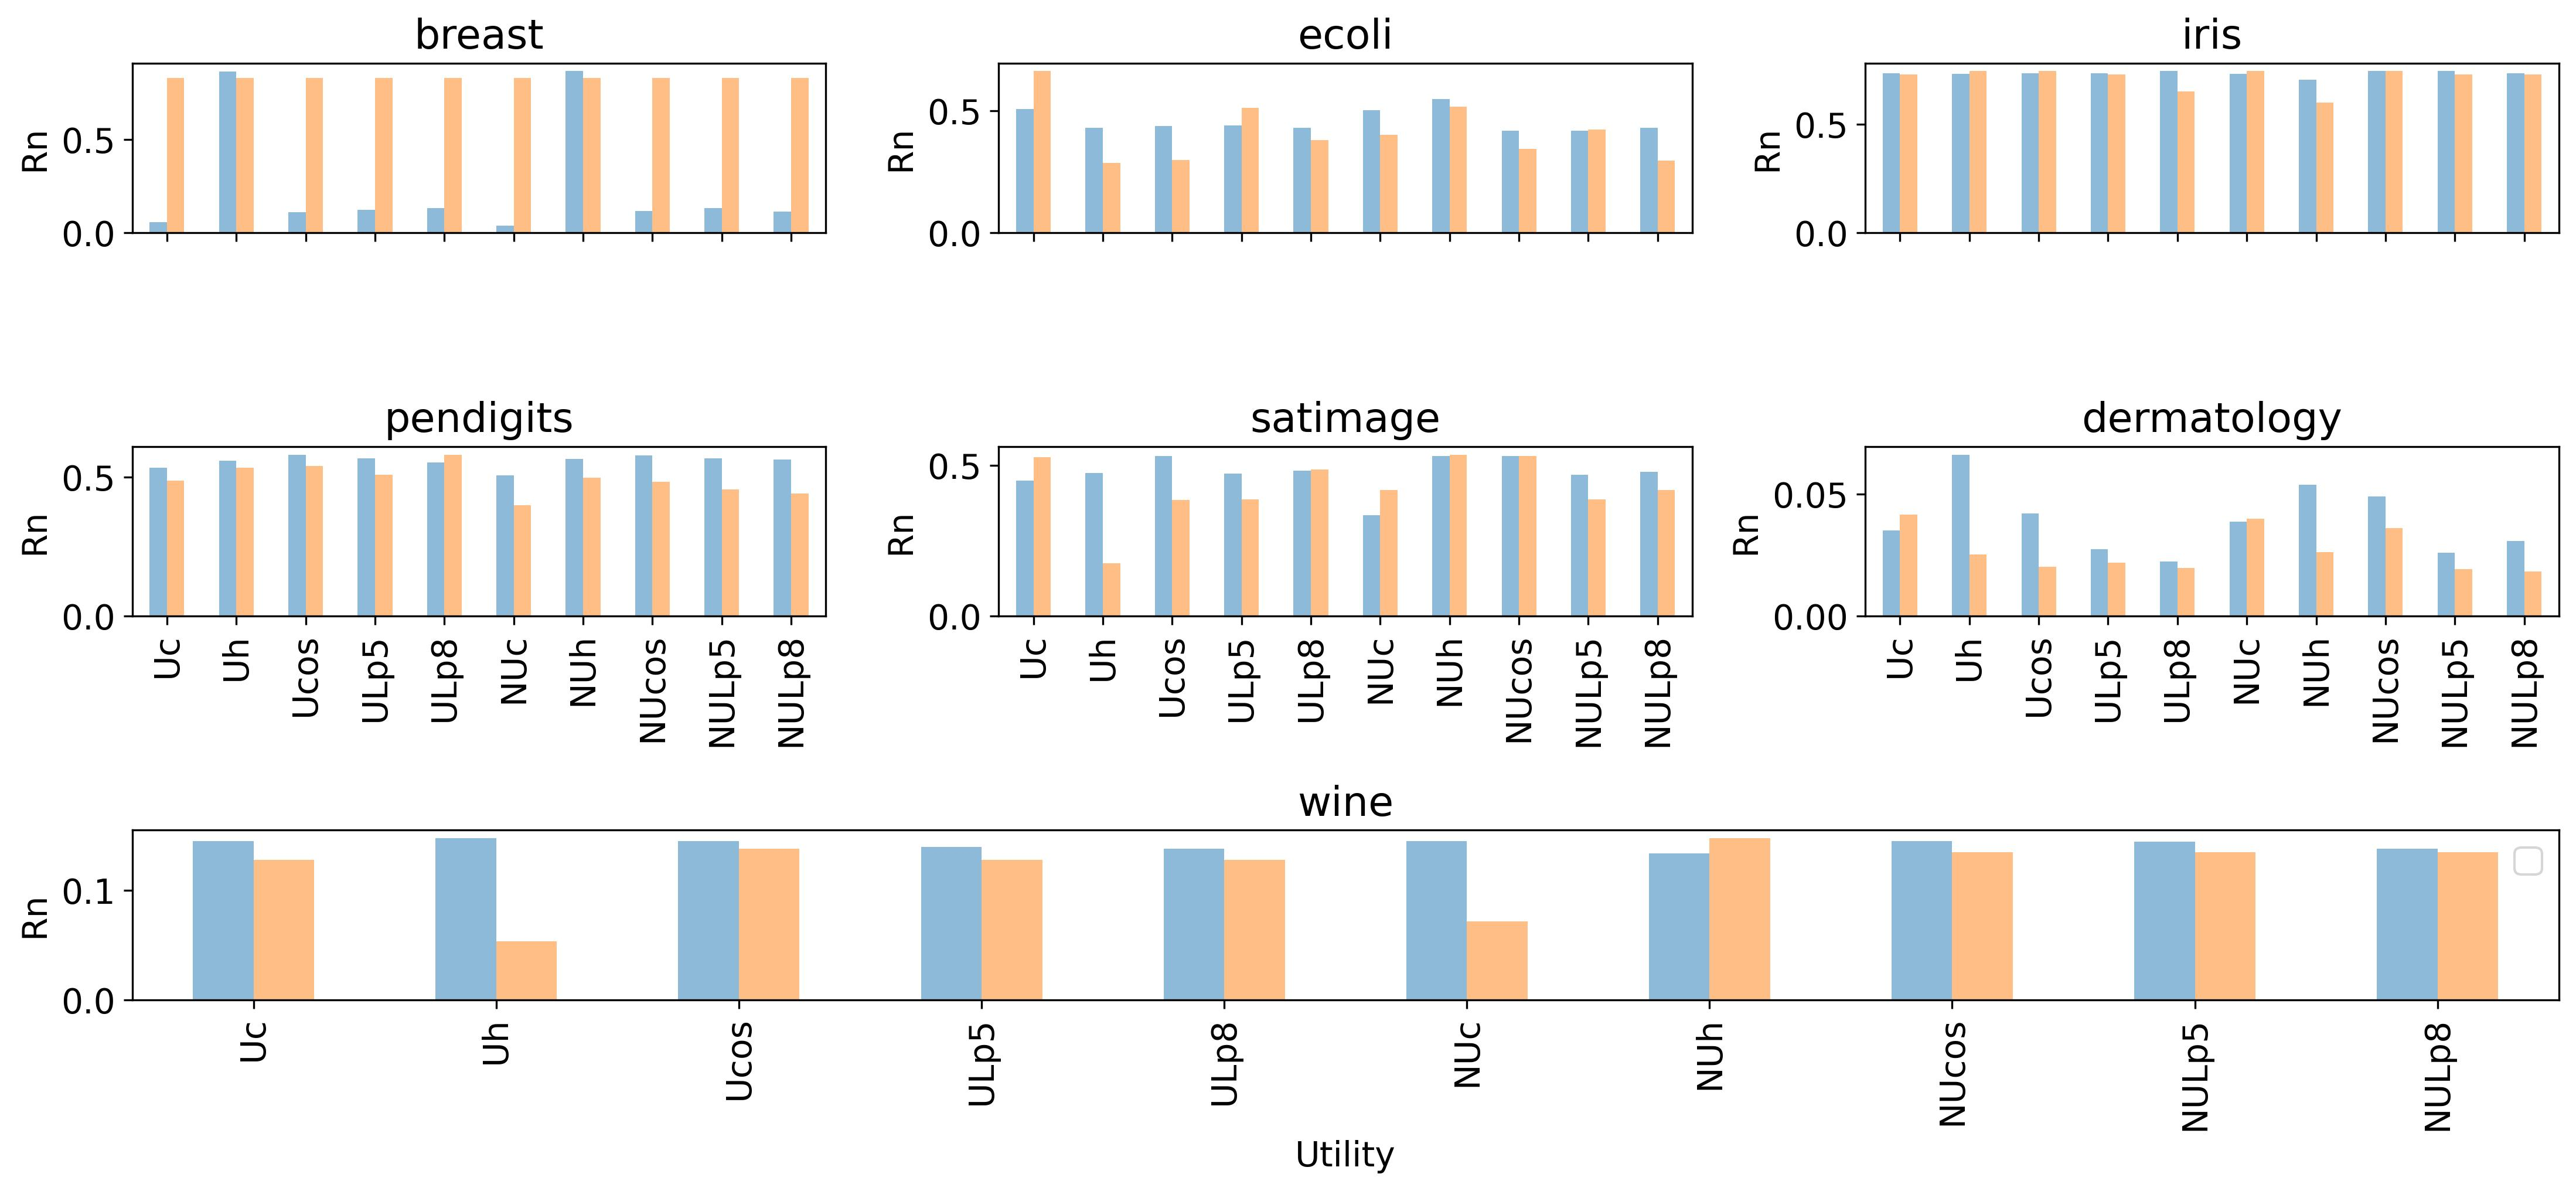
\includegraphics[width=\textwidth]{img/results_comparison_dataset.jpg}
  \caption{Comparison of performance between datasets (blue for original results). Each one with its scale.}
  \label{fig:ari-datasets}
\end{figure*}

\section{Implementation}

The implementation of the algorithm was done in Python. It consists of a main class \textit{ConsensusKMeans} 
that is initialized with the number of clusters, the number of basic partitionings and the utility function type.

The main method of the class is \textit{fit}, which receives the binary dataset, together with some information about the 
basic partitions (labels and numbers of clusters). Centroids are initialized using random pick from $X^{(b)}$ and, iteratively, 
the algorithm updates the centroids and the labels using as point-to-centroid function the $f$ function corresponding to the utility
function used. The algorithm stops when the sum of these distances (inertia) do not change below a tolerance (default $10^{-10}$) or a
maximum number of iterations (default 1000) is reached. However, convergency occurs in less than 15 iterations in most cases.

The $f$ function is calculated using vectorized operations. For euclidean, cosine and p-distances, the use of \textit{scipy} library and
its \textit{cdist} function were key to achieve good performance. In the case of the KL-divergence, the function was implemented from scratch
using numpy operations and broadcasting. Previous attempts calculating the point-to-centroid function using loops were not efficient, taking
more than 10 times the time of the vectorized version, whichm given the number of iterations, was not acceptable. The version of $f$ for the
normalized utility function was implemented in a similar way but weighting each point-to-centroid distance with the inverse of $\mu$.

The algorithm was tested using the datasets from the UCI repository. The results of the clustering were evaluated using the Adjusted Rand Index (ARI).


\section{Results}

The results of the algorithm were compared with the original results of the paper. The ARI was calculated for each dataset and each utility function. 
The results are shown in Tables \ref{table:combined-results-us} and \ref{table:combined-results-nus}. The results are also shown in Figures 
\ref{fig:ari-datasets} and \ref{fig:ari-metrics} for each dataset and utility function.

The results show that the new implementation of the algorithm is consistent with the original results. It can be seen that there are significant
differences in \textit{breast} and \textit{dermatology} datasets. In the first one, ours outperforms the original implementation in 8 out of 10 
utility functions. However, in the second one, the original implementation outperforms ours in 7 out of 10. One of the reasons for this could be
that both datasets had missing values, but in ~\cite{Original} the authors didn't specify how did they handle them. In our case, we used the simplest
approach, which is imputing all of them with zeros, so that we can be as fair as possible with the original implementation without removing any data.

We can see as well that there's a systematic difference in the results of the \textit{ecoli} dataset. The ARI is always higher in the original implementation.
The authors specify that they deleted two clusters containing only one point, but they don't specify which ones. We didn't do any handmade postprocessing
in order to have a generic framework, so we didn't delete any cluster. This could be the reason for the difference in the results.

When analyzing the results by utility function, we can see that the results are consistent with the original ones. In Figure \ref{fig:ari-metrics},
in some cases as for $U_{cos}$, $U_{L5}$ and $U_{L8}$, in the normalized version some discrepancies in the results are not appearing. In Figure \ref{fig:ari-statistics}
no significative differences are observed in the average ARI for each utility function. The distribution of the ARI for each dataset is also consistent with the original
results.

The training time for the algorithm was also measured for each dataset and utility function. The comparison is shown in Table \ref{tab:time_values_per_dataset}. From the
results we can see that, in general, the training time is consistent with the original results but ours is significantly higher
in the case of \textit{dermatology}, for which it goes from 1.26 seconds to 11.81. However, it's important to note that the times for \textit{satimage} are similar
even when the number of points is 4435 in the original paper and 6435 in our case.

\begin{table*}[t!]
  \centering
  \begin{tabular}{l|ccccccccccc}
  \toprule
   & breast & ecoli & iris & pendigits & satimage & dermatology & wine \\
  \midrule
  Original ($U_c$) & 1.95 & 1.40 & 0.33 & 81.19 & 32.47 & 1.26 & 0.56 \\
  Results ($U_c$) & 1.72 & 2.70 & 0.48 & 111.18 & 33.78 & 11.81 & 2.75 \\
  \bottomrule
  \end{tabular}
  \caption{Training times values for each dataset.}
  \label{tab:time_values_per_dataset}
  \end{table*}

% Insert plot
\begin{figure*}[h]
  \centering
  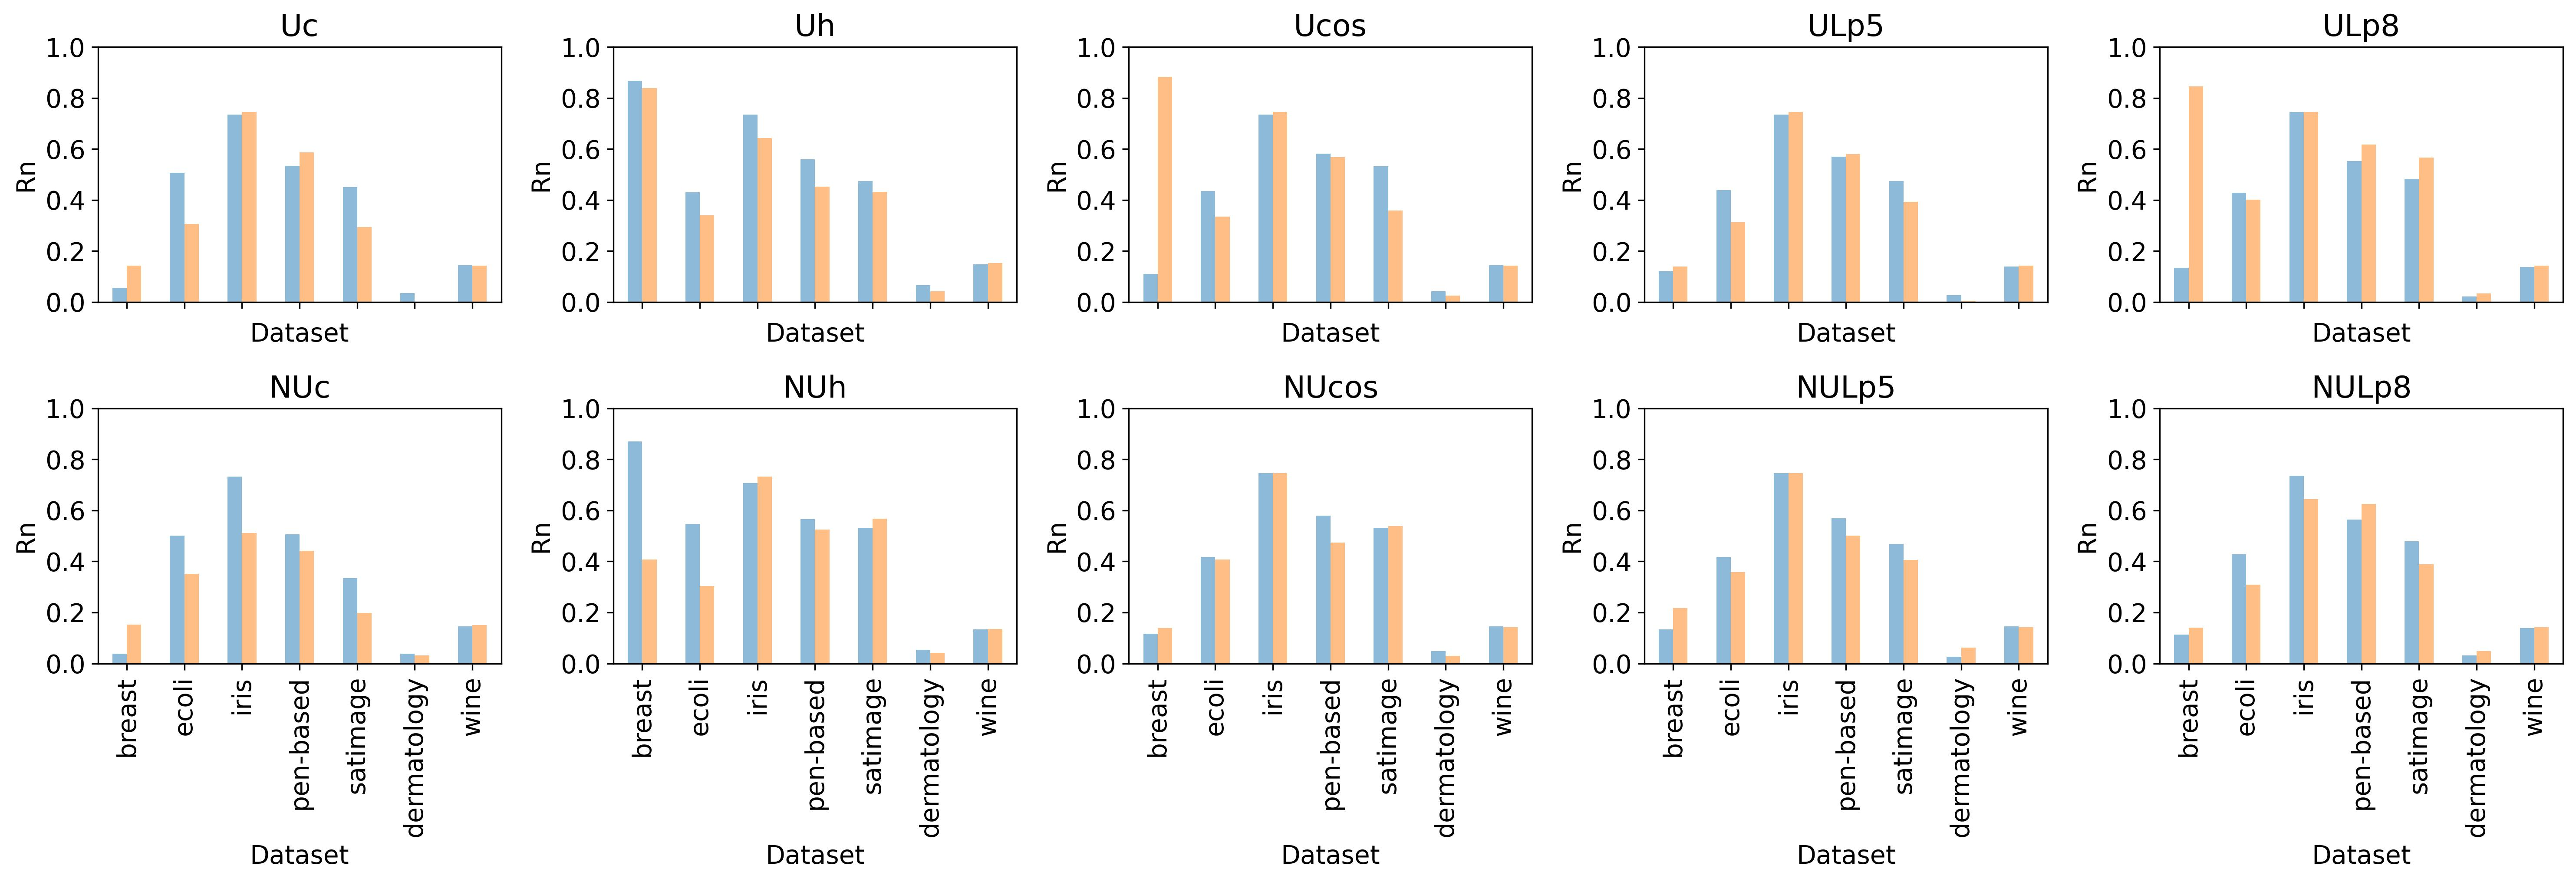
\includegraphics[width=\textwidth]{img/results_comparison_metric.jpg}
  \caption{Comparison of performance by metrics (blue for original results). All of them in the same scale.}
  \label{fig:ari-metrics}
\end{figure*}

% Insert plot
\begin{figure*}[h]
  \centering
  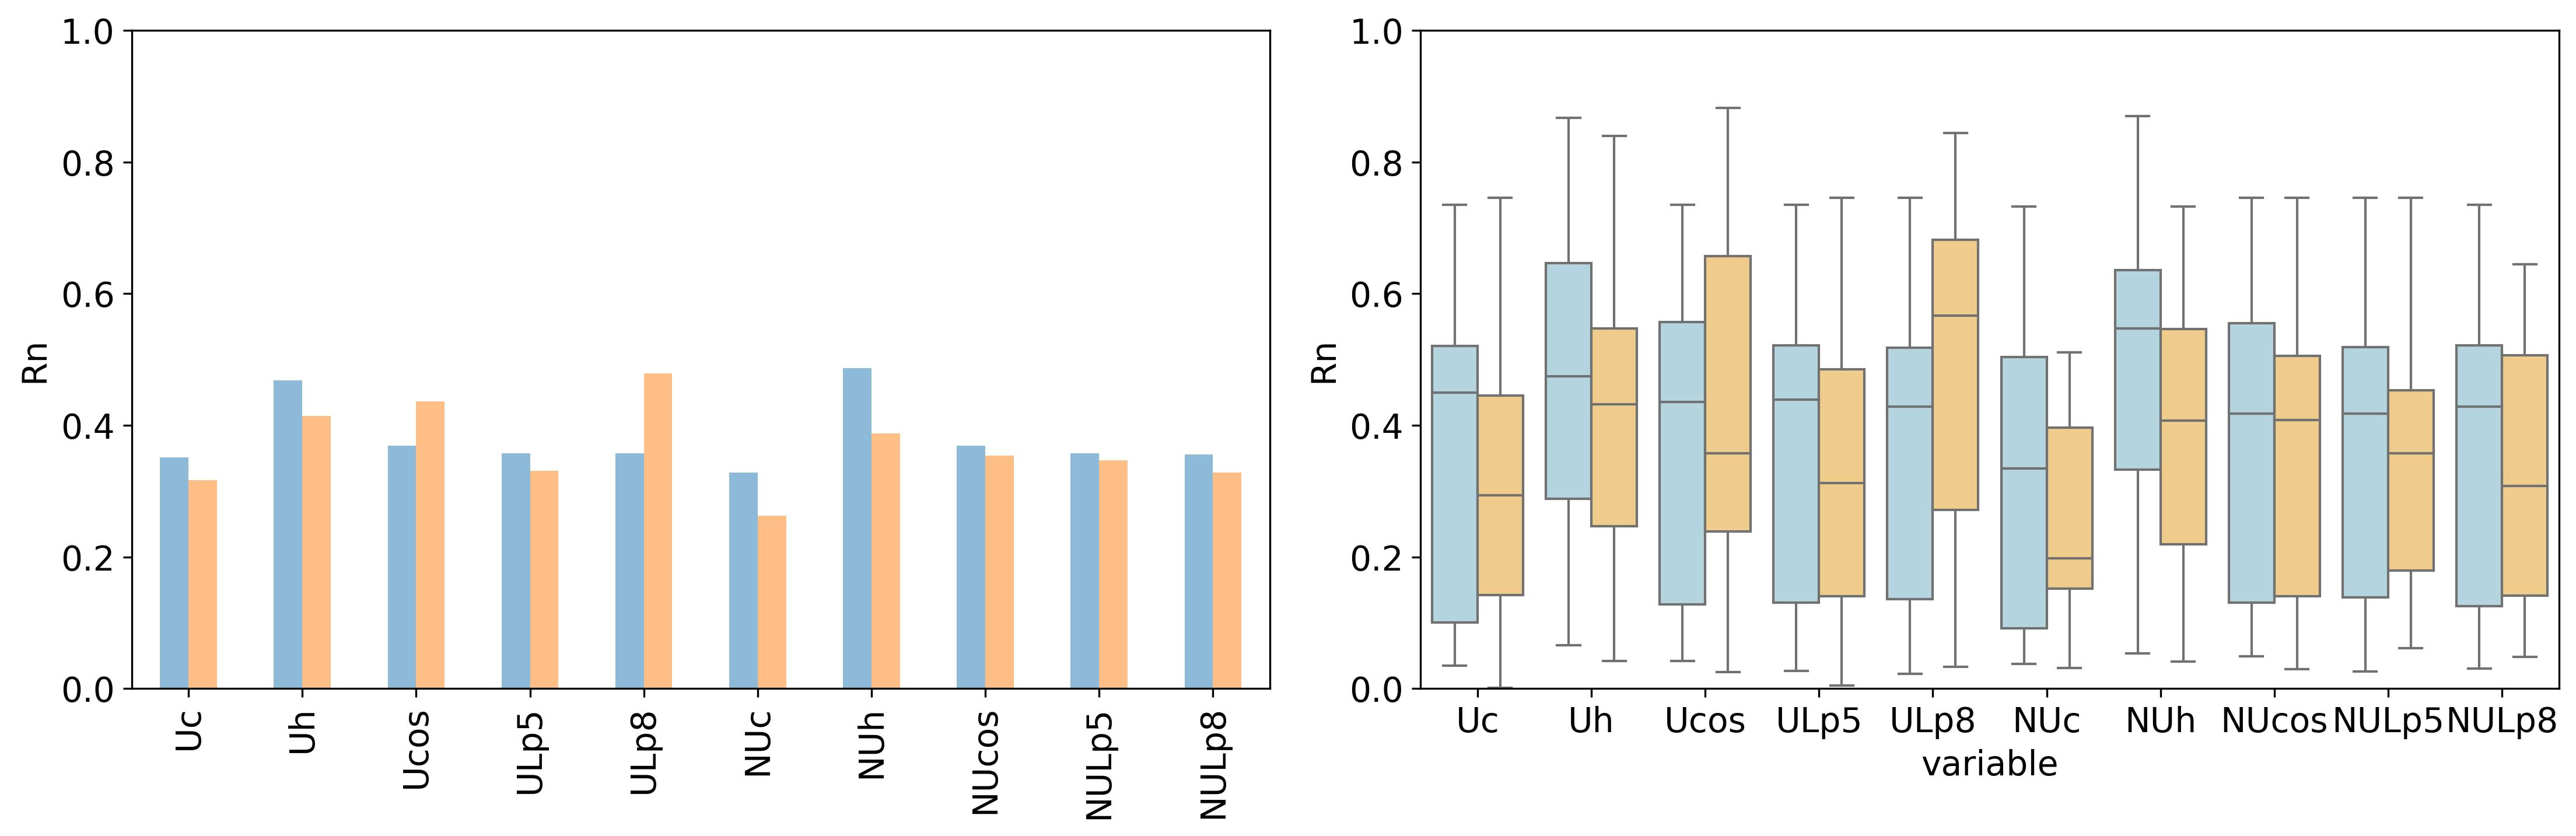
\includegraphics[width=\textwidth]{img/compare_metrics_distribution.jpg}
  \caption{Comparison of statistical performance by metrics (blue for original results) across all the datasets. 
  Average comparison in the left. Distribution for each dataset in the right.}
  \label{fig:ari-statistics}
\end{figure*}

\begin{table*}[h]
  \centering
  \begin{tabular}{l|cc|cc|cc|cc|cc}
    \hline
    & \multicolumn{2}{c|}{$U_c$} & \multicolumn{2}{c|}{$U_H$} & \multicolumn{2}{c|}{$U_{\cos}$} & \multicolumn{2}{c|}{$U_{L5}$} & \multicolumn{2}{c}{$U_{L8}$} \\
    \hline
    & Original & Results & Original & Results & Original & Results & Original & Results & Original & Results \\
    \hline
    breast & 0.0556 & 0.1427 & 0.8673 & 0.8392 & 0.1111 & 0.8825 & 0.1212 & 0.1387 & 0.1333 & 0.8445 \\
    ecoli & 0.5065 & 0.3052 & 0.4296 & 0.3405 & 0.4359 & 0.3350 & 0.4393 & 0.3119 & 0.4284 & 0.4019 \\
    iris & 0.7352 & 0.7455 & 0.7338 & 0.6423 & 0.7352 & 0.7455 & 0.7352 & 0.7455 & 0.7455 & 0.7455 \\
    pendigits & 0.5347 & 0.5858 & 0.5596 & 0.4520 & 0.5814 & 0.5679 & 0.5692 & 0.5791 & 0.5527 & 0.6174 \\
    satimage & 0.4501 & 0.2934 & 0.4743 & 0.4322 & 0.5322 & 0.3579 & 0.4738 & 0.3920 & 0.4834 & 0.5667 \\
    dermatology & 0.0352 & 0.0016 & 0.0661 & 0.0419 & 0.0421 & 0.0252 & 0.0274 & 0.0051 & 0.0223 & 0.0332 \\
    wine & 0.1448 & 0.1421 & 0.1476 & 0.1524 & 0.1448 & 0.1421 & 0.1397 & 0.1449 & 0.1379 & 0.1421 \\
    \hline
  \end{tabular}
  \caption{KCC Clustering Results (by Rn) (Us)}
  \label{table:combined-results-us}
  \centering
  \begin{tabular}{l|cc|cc|cc|cc|cc}
    \hline
    & \multicolumn{2}{c|}{$NU_c$} & \multicolumn{2}{c|}{$NU_H$} & \multicolumn{2}{c|}{$NU_{\cos}$} & \multicolumn{2}{c|}{$NU_{L5}$} & \multicolumn{2}{c}{$NU_{L8}$} \\
    \hline
    & Original & Results & Original & Results & Original & Results & Original & Results & Original & Results \\
    \hline
    breast & 0.0380 & 0.1519 & 0.8694 & 0.4067 & 0.1173 & 0.1387 & 0.1329 & 0.2170 & 0.1126 & 0.1410 \\
    ecoli & 0.5012 & 0.3515 & 0.5470 & 0.3045 & 0.4179 & 0.4081 & 0.4174 & 0.3574 & 0.4281 & 0.3080 \\
    iris & 0.7325 & 0.5111 & 0.7069 & 0.7323 & 0.7455 & 0.7455 & 0.7455 & 0.7455 & 0.7352 & 0.6444 \\
    pendigits & 0.5060 & 0.4419 & 0.5652 & 0.5253 & 0.5789 & 0.4736 & 0.5684 & 0.5004 & 0.5639 & 0.6250 \\
    satimage & 0.3349 & 0.1979 & 0.5323 & 0.5675 & 0.5318 & 0.5377 & 0.4691 & 0.4065 & 0.4797 & 0.3883 \\
    dermatology & 0.0386 & 0.0317 & 0.0537 & 0.0415 & 0.0490 & 0.0300 & 0.0259 & 0.0617 & 0.0309 & 0.0481 \\
    wine & 0.1448 & 0.1513 & 0.1336 & 0.1348 & 0.1449 & 0.1421 & 0.1447 & 0.1421 & 0.1379 & 0.1421 \\
    \hline
  \end{tabular}
  \caption{KCC Clustering Results (by Rn) (NUs)}
  \label{table:combined-results-nus}
\end{table*}  

% Conclusions
\section{Conclusions}

In conclusion, this work successfully implemented and evaluated the K-means-based Consensus Clustering algorithm proposed by Wu et al.~\cite{Original}. 
The algorithm, designed to obtain a stable consensus clustering from multiple K-Means clusterings, was thoroughly examined and 
tested using datasets from the UCI repository.

The primary objective of the algorithm is to find a consensus partitioning that aligns with a set of basic partitionings obtained 
through repeated application of the K-means algorithm. The paper establishes a mathematical framework, introducing utility functions
and demonstrating their correspondence with K-Means loss functions. This mapping allows the consensus clustering problem to be efficiently 
solved using the K-Means algorithm.

The experimental setup closely followed the methodology outlined in the original paper, utilizing UCI datasets and generating basic
partitionings through repeated K-means applications. Various utility functions were tested, both in their original and normalized 
versions, with the consensus clustering algorithm performing consistently across different datasets.

The implementation of the algorithm in Python demonstrated efficiency and accuracy. The results were evaluated using the Adjusted 
Rand Index (ARI), and the algorithm's performance was compared with the original paper's results. Overall, the implemented algorithm 
produced comparable results, maintaining consistency across different utility functions and datasets.

While discrepancies were observed in specific datasets, such as \textit{breast} and \textit{dermatology}, these differences could 
be attributed to variations in handling missing values and the presence of clusters with a single point. The systematic difference 
in the \textit{ecoli} dataset was identified as a result of cluster deletion in the original paper, a step not replicated in the current
implementation to maintain generality. With respect to training times, the implemented algorithm was slower than the original in
some cases, particularly for the \textit{dermatology} dataset. However, the magnitudes are similar.

In summary, the implemented K-means-based Consensus Clustering algorithm demonstrates robustness and reliability in generating 
consensus clusterings from diverse datasets. The alignment with the original paper's results, along with the flexibility 
to accommodate different utility functions, underscores the algorithm's utility in practical clustering applications.
  

\newpage
% \begin{samepage}
  \begin{thebibliography}{40}
    \addcontentsline{toc}{chapter}{Bibliograf\'ia}
   {\footnotesize
   \bibitem{Original} J. Wu, H. Liu, H. Xiong, J. Cao and J. Chen, "K-Means-Based Consensus Clustering: A Unified View," in IEEE Transactions on Knowledge and Data Engineering, vol. 27, no. 1, pp. 155-169, 1 Jan. 2015, doi: 10.1109/TKDE.2014.2316512.
   keywords: {Clustering algorithms;Linear programming;Partitioning algorithms;Convex functions;Robustness;Educational institutions;Vectors;Consensus clustering;K-means;utility function},
     
   }
   
   \end{thebibliography}
% \end{samepage}

  
\end{document}




